% !TeX root = 00main.tex

%%%%%%%%%%%%%%%%%%%%%%%%%%%%%%%%%%%%%%%%%%%%%%%%%%%%%%%%%%%%%%%%%%%%%%%%%%%
% System design
%%%%%%%%%%%%%%%%%%%%%%%%%%%%%%%%%%%%%%%%%%%%%%%%%%%%%%%%%%%%%%%%%%%%%%%%%%%

\subsection*{Nanopulser head}

\subsection*{Control box}

One symptom of a blown fuse can be that  the pulser does communicate but either does not produce light, or produces a smaller, wide pulse.


\subsection*{Cable design}


The ethernet cables should {\bf never} be unplugged from the box, while the power is on, as the power for both the digital electronics, as well as for the pulser circuits runs through them. Accidental hot-swapping can result in one of the fuses blowing. 

\subsubsection*{Connection box}

\begin{figure}
\begin{center}	
  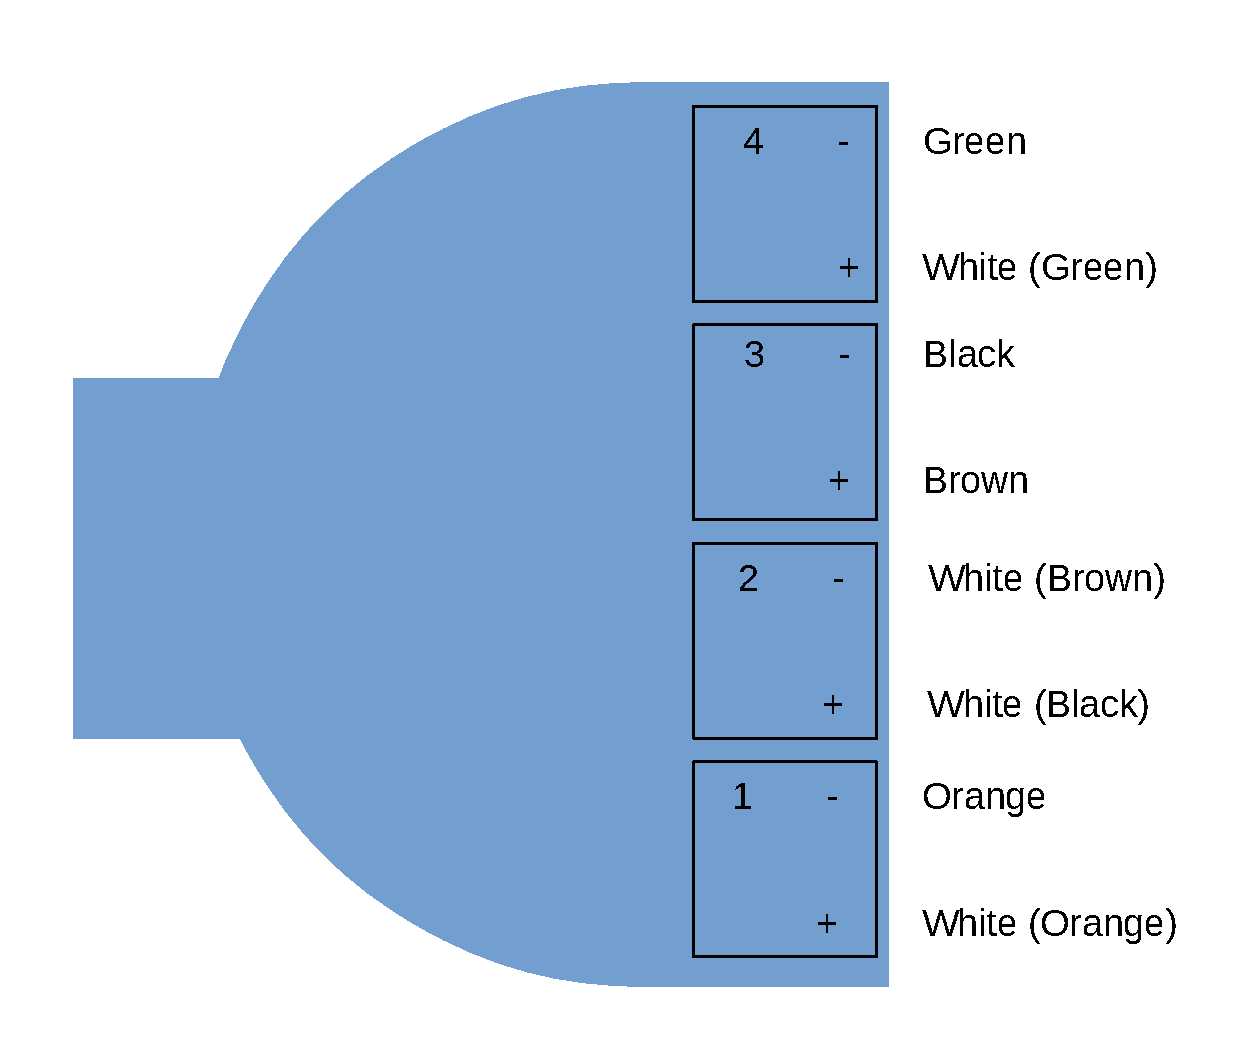
\includegraphics[width=0.5\linewidth]{figures/connector.pdf}
  \caption{A diagram indication how the eight-way connector should be connected to the cables going into the vessel.}
  \label{figure:connector}
\end{center}
\end{figure}

At the final installation, the cables should be wrapped with a tie-wrap inside the junction box, to avoid damage to the connection by accidentally pull the cables.
